% *********************************************************************
% © 2016–2025 Jeremy Sylvestre
%
% Permission is granted to copy, distribute and/or modify this document
% under the terms of the GNU Free Documentation License, Version 1.3 or
% any later version published by the Free Software Foundation; with no
% Invariant Sections, no Front-Cover Texts, and no Back-Cover Texts. A
% copy of the license is included in the appendix entitled “GNU Free
% Documentation License” that appears in the output document of this
% PreTeXt source code. All trademarks™ are the registered® marks of
% their respective owners.
%
% *********************************************************************
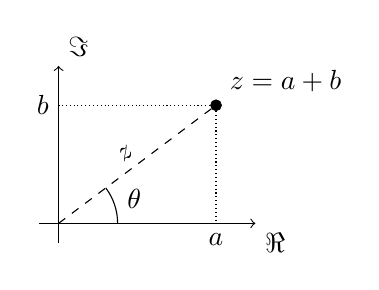
\begin{tikzpicture}[
	point/.style={circle,draw,very thin,fill,inner sep=0pt,minimum size=4pt},
]
	\draw[->] (-0.25,0) to (2.5,0) node[below right] {$\Re$};
	\draw[->] (0,-0.25) to (0,2) node[above right] {$\Im$};

	\node[point] at (2,1.5) (z) [label=above right:{$z = a + b \ci$}] {};

	\draw[densely dotted] (z) to (2,0) node[below] {$a$} ;
	\draw[densely dotted] (z) to (0,1.5) node[left] {$b$};
	\draw[dashed] (0,0) to node[above,sloped] {$\cmodulus{z}$} (z);

	\draw (0,0) ++(0:0.75cm) arc (0:36.87:0.75cm) node[midway,xshift=0.25cm,yshift=0.08cm] {$\theta$};

\end{tikzpicture}
